
\subsection{Data Description}
We describe our three distinct data sources here as well as the details associated with linking them together. First, we describe the matched employer-employee data from \ac{RAIS}. Second, we describe our data on management practices from the \ac{WMS}. Third, we describe our data on firm output and non-labor inputs from the \ac{PIA}. Finally, we describe our the linked datasets used in our analysis.

\subsection{Wage Decomposition Details}


%Ian M. Schmutte
% 2018 Aug 4
%source /projects/schmutte/MGMT/MGMT_source/data/_dev/programs/prepare/02_run_CG/CG_est_twfe_exp_normalized.(m,log)

\begin{table}
  \label{tab:AKM_vardecomp}
  \small 
   \caption{Decomposition of Variance in Log Wages: RAIS 2003-2013}
   \begin{center}
      \begin{tabular}{l c k r}
      \toprule            
                                      &\quad \quad & \multirow{1}{*}{Variance}  & \multirow{1}{*}{Share}  \\
                                      & & \multirow{1}{*}{Component} &  \multirow{1}{*}{of Total}\\
\midrule
      Log Wage Var.              & & $ 0.472$   &    $100.0\%$         \\  
      Variance Components:                     &&            &                      \\ 
      \quad $\var(\text{Worker Effect~}\theta)$  & & $ 0.235$   &   $ 49.8\% $         \\
      \quad $\var(\text{Estab. Effect~} \psi)$    && $ 0.088$   &   $ 18.5\% $         \\
      \quad $\var(X\beta)$                        && $ 0.046$   &   $ 9.7\% $          \\
      \quad $\var(\text{Residual})$               && $0.044$    &   $ 9.2\% $          \\
      \quad $2\times \cov(\theta,\psi)$           && $0.095$    &   $20.2\%$           \\
      \quad $2\times \cov(X\beta,\theta)$         && $-0.034$   &   $-7.3\%$           \\
      \quad $2\times \cov(X\beta,\psi)$           && $-0.001$    &   $-0.0\%$           \\
  \bottomrule
   \end{tabular}
   \end{center}
   \label{tab:AKM_vardecomp}
   \footnotesize{Notes: Share of variance in log wages explained by components estimated from the AKM model described in Equation \eqref{eq:AKM_full}.}
\end{table}       

% Ian M. Schmutte
% AKM_corr.tex
% This version: 4 Aug 2018
% Correlation table of estimated components from AKM estimation
%SOURCE: Dropbox\MGMT_source\data\_dev\programs\prepare\03.01.post_CG_data_read.lst


\begin{table}[h t]
	\caption{Correlation among log wage components from AKM model: RAIS 2003--2013 \label{tab:AKM_corr}}
	\begin{center}
	\begin{tabular}{c l k k k k k k k}																					
		\toprule																					
			&		&		&		&	\multicolumn{5}{c}{Component Correlations}													\\ \cline{5-9} \noalign{\smallskip}
		Component	&	Label	                                &	\m{Mean}	&	\m{Std. Dev.}	&	\m{$Y$}	&	\m{$X\hat{\beta}$}	&	\m{$\hat{\theta}$}	&	\m{$\hat{\psi}$}	&	\m{$\hat{\varepsilon}$}	\\	
		\midrule
		$Y$	&	Log wage 	                                    &	1.649	&	0.687	&	1.000	&		    &		    &  		    &		    \\	
		$X\hat{\beta}$	&	Time varying characteristics$^\dag$	&	0.137	&	0.215	&	0.192	&	1.000	&		    &		    &    		\\	
		$\hat{\theta}$	&	Worker effect	                    &	0.000	&	0.485	&	0.797	&  -.166	&	1.000	&		    &   		\\	
		$\hat{\psi}$	&	Firm effect             	        &	0.000	&	0.296	&	0.663	&	-.009	&	0.332	&	1.000	&			\\
		$\hat{\varepsilon}$	&	Sample residual	                &	0.000	&	0.209	&	0.304	&	0.000	&	0.000	&	0.000	&	1.000	\\
		\bottomrule
	\end{tabular}
	\end{center}
	\footnotesize{Notes: Observation-weighted correlations among the variance components of log wages estimated from the AKM model described in Equation \eqref{eq:AKM_full}}

\end{table}

	



\subsection{Productivity Analysis}

\begin{figure}[h]
\centering
\fbox{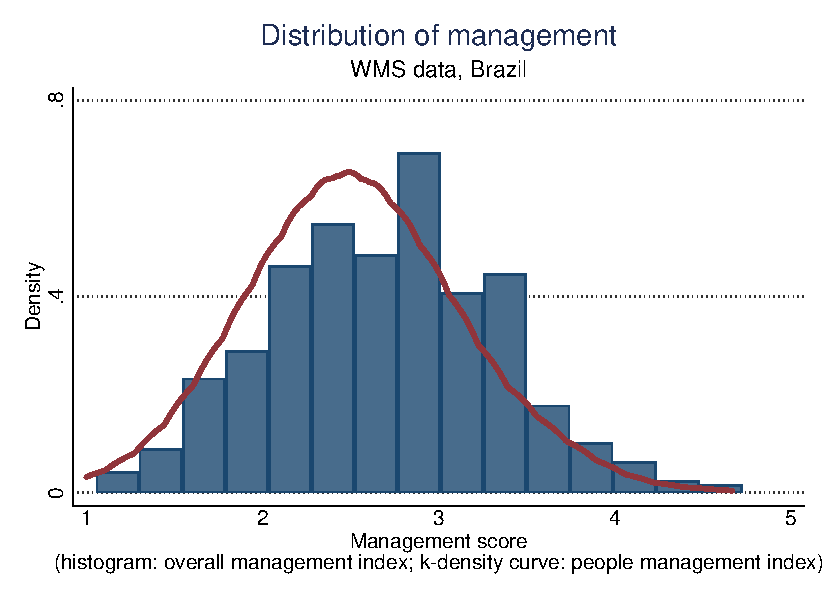
\includegraphics{../figures/mgmtscor_hist}}
\caption{Distribution of firm management z-score from WMS }
\label{fig:mgmtscor_hist}
\end{figure}


\begin{landscape}
% \newpage
\begin{figure}[h]
\centering
\includegraphics[width=1.4\textwidth]{../figures/fe_mgmt_summ}
\caption{plant-specific starting pay effect by plant management z-score}
\label{fig:mgmt_v_fe}
\end{figure}
\end{landscape}


\begin{landscape}
\begin{figure}[h]
\centering
\includegraphics[width=1.4\textwidth]{../figures/pe_mgmt_summ}
\caption{worker-specific effect by plant management z-score}
\label{fig:mgmt_v_fe}
\end{figure}
\end{landscape}

\clearpage
\begin{figure}[h]
\centering
\includegraphics{../figures/fe_v_sales}
\caption{Log sales per worker by plant-specific starting wage premium, $\hat{\psi}$}
\label{fig:fe_v_sales}
\end{figure}

% EMPLOYMENT SHARES FIGURE
\begin{figure}[h]
	\centering
	\fbox{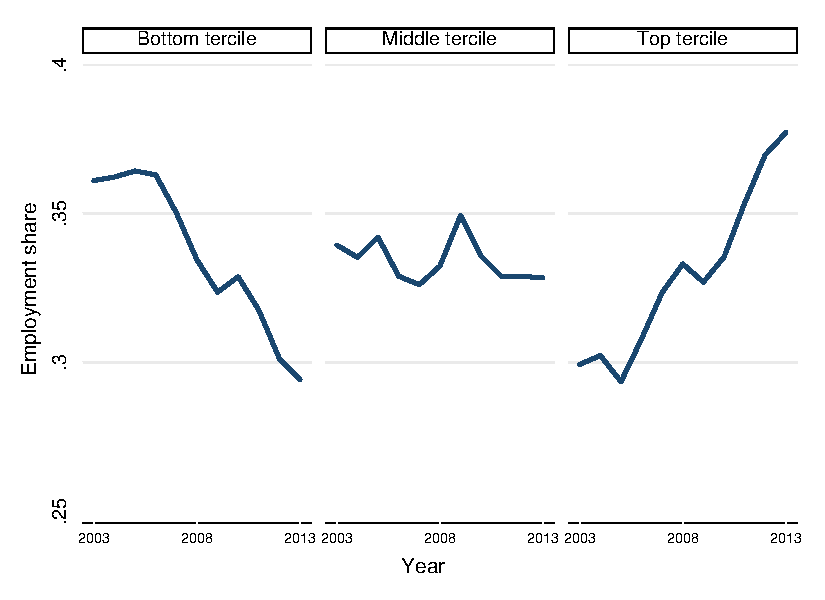
\includegraphics{./exhibits/fig_emp_shares}}
	\caption{Employment shares by management tercile, 2003-2013}
	\label{fig:emp_shares}
\end{figure}



\begin{landscape}
%\scalebox{0.95}{
	\begin{table}
	\caption{Difference in means between WMS-RAIS merged firms and non-WMS firms, 50+ employees} \label{tab:wms_diff_50}
	\small
	\singlespace
	\input{../tables/wms_rais_diff}
	\tablenotes{\textbf{Notes:} This table compares the firms in the WMS sample and the overall RAIS sample for firms with more than 50 employees. The WMS sample from 2008 is a random sample of firms between 100-5000 workers, and the 2013 sample was stratified to include 20\% of firms in the 50-99 employees category and the remaining 80\% of the sample in the 100-5000 sample.}
	\end{table}
%}
\end{landscape}

\clearpage
\begin{landscape}
%\scalebox{0.95}{
	\begin{table}
	\caption{Difference in means between WMS-RAIS merged firms and non-WMS firms, 100+ employees} \label{tab:wms_diff_100}
	\small
	\singlespace
	\input{../tables/wms_rais_diff_100p}
	\tablenotes{\textbf{Notes:} This table compares the firms in the WMS sample and the overall RAIS sample for firms with more than 50 employees. The WMS sample from 2008 is a random sample of firms between 100-5000 workers, and the 2013 sample was stratified to include 20\% of firms in the 50-99 employees category and the remaining 80\% of the sample in the 100-5000 sample. }
	\end{table}
	%}
\end{landscape}

	\begin{table}
	\caption{RAIS, Orbis and interviewed sample differences: key variable means}
	\small
	\singlespace
	\center
	\hline
	~ \\
	\textbf{2008}
	\input{../tables/sf_compare2008} \\
	~ \\
	\textbf{2013}
	\input{../tables/sf_compare2013}
	\tablenotes{\textbf{Notes:} This table includes all firms in the RAIS sampling frames, and compares RAIS key variables across the sample of firms that (a) are only in RAIS and not in the Orbis universe ("Not in Orbis"); (b) are in RAIS/Orbis universes but not in the WMS sampling frame ("Not in frame"), (c) are in RAIS/Orbis universes and in the WMS random sample of firms but were not selected to be in , and (d) are in the RAIS/Orbis universes, in the WMS sample. The ``plant size category'' comes from RAIS, and ``5'' indicates firms with between 50--99 employees. Code ``6'' indicates 100--249. Code ``7'' indicates 250--499. Code ``8'' indicates 500--999. Code ``9'' indicates firms with 1000 or more employees.}
	\end{table}


\begin{landscape}
\begin{table}
	\caption{Worker FE (mean) vs management}
	\label{tab:zpe}
	\small
	\singlespace
	\center
\scalebox{0.9}{	
	\input{../../data/analysis/output/tables/zpe.tex}} \\
	~ \\
	\tablenotes{\textbf{Notes:} *** indicates significance at the 1\% level, ** at the 5\% level, and * at the 10\% level. All standard errors are clustered by plant. Management score, production worker average fixed effect, and manager average fixed effect are standardized. All columns control for industry. In addition, the indicated columns also control for state, private ownership, number of competitors, union share, firm age, share male, average work hours, share white, and whether the firm is a multinational.  }
	
\end{table}
\end{landscape}

\begin{landscape}
\begin{table}
	\caption{Worker FE Production Workers vs management}
	\label{tab:zpe_prod}
	\small
	\singlespace
	\center
\scalebox{0.75}{	
	\input{../../data/analysis/output/tables/zpe_labr.tex}} \\
	~ \\
	\tablenotes{\textbf{Notes:} *** indicates significance at the 1\% level, ** at the 5\% level, and * at the 10\% level. All standard errors are clustered by plant. Management score, production worker average fixed effect, and manager average fixed effect are standardized. All columns control for industry. In addition, the indicated columns also control for state, private ownership, number of competitors, union share, firm age, share male, average work hours, share white, and whether the firm is a multinational.  }
	
\end{table}
\end{landscape}


\begin{landscape}
\begin{table}
	\caption{Worker FE Managers vs management}
	\label{tab:zpe_mngr}
	\small
	\singlespace
	\center
\scalebox{0.7}{	
	\input{../../data/analysis/output/tables/zpe_mngr.tex}} \\
	~ \\
	\tablenotes{\textbf{Notes:} *** indicates significance at the 1\% level, ** at the 5\% level, and * at the 10\% level. All standard errors are clustered by plant. Management score, production worker average fixed effect, and manager average fixed effect are standardized. All columns control for industry. In addition, the indicated columns also control for state, private ownership, number of competitors, union share, firm age, share male, average work hours, share white, and whether the firm is a multinational.  }
	
\end{table}
\end{landscape}


\clearpage
\begin{landscape}
\begin{table}
	\caption{Firm FE vs management}
	\label{tab:zfe}
	\small
	\singlespace
	\center
\scalebox{0.9}{	
	\input{../../data/analysis/output/tables/zfe.tex}} \\
	~ \\
	\tablenotes{\textbf{Notes:} *** indicates significance at the 1\% level, ** at the 5\% level, and * at the 10\% level. All standard errors are clustered by plant. Management score, production worker average fixed effect, and manager average fixed effect are standardized. All columns control for industry. In addition, the indicated columns also control for state, private ownership, number of competitors, union share, firm age, share male, average work hours, share white, and whether the firm is a multinational. }
	
\end{table}
\end{landscape}


\clearpage
%\begin{landscape}
\begin{table}
	\caption{Manager FE vs people management}
	\label{tab:zpe_mngr_ppl}
	\small
	\singlespace
	\center
\scalebox{0.9}{	
	\input{../../data/analysis/output/tables/zpe_mngr_ppl.tex}} \\
	~ \\
	\tablenotes{\textbf{Notes:} *** indicates significance at the 1\% level, ** at the 5\% level, and * at the 10\% level. All standard errors are clustered by plant. Management score, production worker average fixed effect, and manager average fixed effect are standardized. All columns control for industry. In addition, the indicated columns also control for state, private ownership, number of competitors, union share, firm age, share male, average work hours, share white, and whether the firm is a multinational. }
	
\end{table}


\clearpage
%\begin{landscape}
\begin{table}
	\caption{Production worker FE vs people management}
	\label{tab:zpe_labr_ppl}
	\small
	\singlespace
	\center
\scalebox{0.9}{	
	\input{../../data/analysis/output/tables/zpe_labr_ppl.tex}} \\
	~ \\
	\tablenotes{\textbf{Notes:} *** indicates significance at the 1\% level, ** at the 5\% level, and * at the 10\% level. All standard errors are clustered by plant. Management score, production worker average fixed effect, and manager average fixed effect are standardized. All columns control for industry. In addition, the indicated columns also control for state, private ownership, number of competitors, union share, firm age, share male, average work hours, share white, and whether the firm is a multinational. }
	
\end{table}

\clearpage
%\begin{landscape}
\begin{table}
	\caption{Firm FE vs people management}
	\label{tab:zfe_ppl}
	\small
	\singlespace
	\center
\scalebox{0.9}{	
	\input{../../data/analysis/output/tables/zfe_ppl.tex}} \\
	~ \\
	\tablenotes{\textbf{Notes:} *** indicates significance at the 1\% level, ** at the 5\% level, and * at the 10\% level. All standard errors are clustered by plant. Management score, production worker average fixed effect, and manager average fixed effect are standardized. All columns control for industry. In addition, the indicated columns also control for state, private ownership, number of competitors, union share, firm age, share male, average work hours, share white, and whether the firm is a multinational. }
	
\end{table}
%\end{landscape}







